\documentclass{article}
\usepackage{graphicx}
\usepackage{subcaption}

\begin{document}

\begin{figure}

\centering

  \begin{subfigure}[b]{\textwidth}
    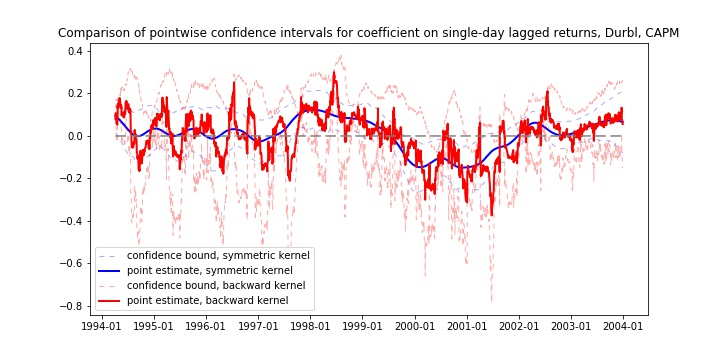
\includegraphics[width=\textwidth]{Durbl/pointwiseCIs_layered_CAPM.jpg}
    \label{fig:1}
  \end{subfigure}
  %
  \begin{subfigure}[b]{0.45\textwidth}
    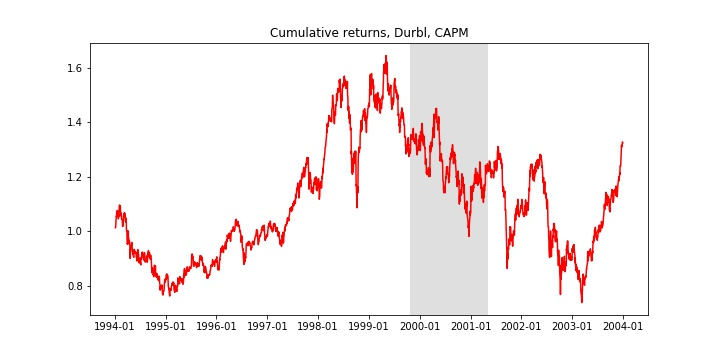
\includegraphics[width=\textwidth]{Durbl/full_cumrets_ofint_CAPM.jpg}
    \caption*{Per. of interest, symmetric kernel}
    \label{fig:2}
  \end{subfigure}
  %
   \begin{subfigure}[b]{0.45\textwidth}
    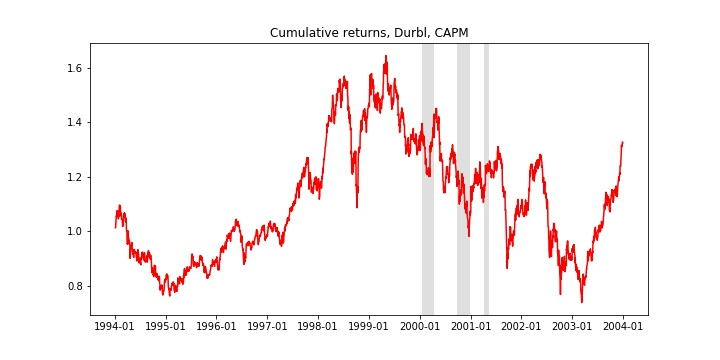
\includegraphics[width=\textwidth]{Durbl/bwunif_full_cumrets_ofint_CAPM.jpg}
    \caption*{Per. of interest, rear-facing kernel}
    \label{fig:2}
  \end{subfigure}
  
\end{figure}

\newpage

\begin{figure}

\centering

  \begin{subfigure}[b]{\textwidth}
    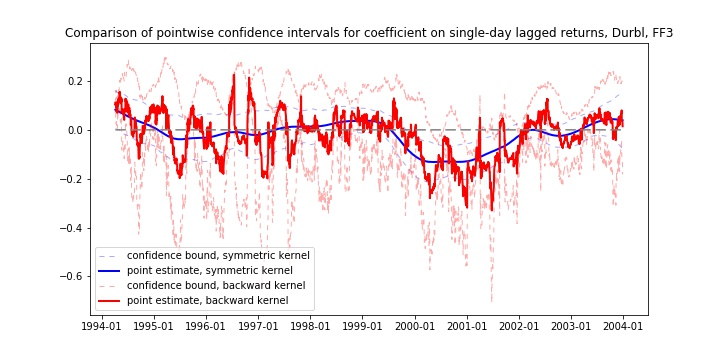
\includegraphics[width=\textwidth]{Durbl/pointwiseCIs_layered_FF3.jpg}
    \label{fig:1}
  \end{subfigure}
  %
  \begin{subfigure}[b]{0.45\textwidth}
    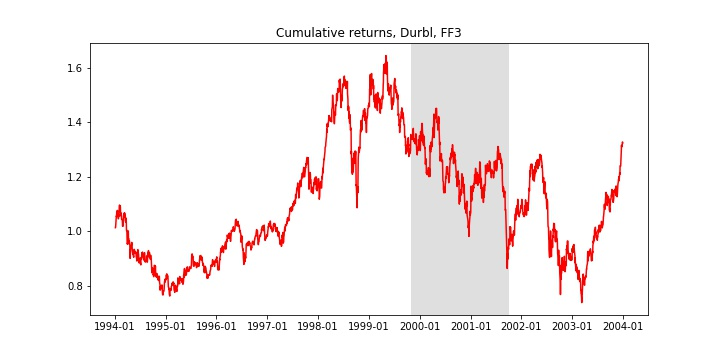
\includegraphics[width=\textwidth]{Durbl/full_cumrets_ofint_FF3.jpg}
    \caption*{Symmetric kernel}
    \label{fig:2}
  \end{subfigure}
  %
   \begin{subfigure}[b]{0.45\textwidth}
    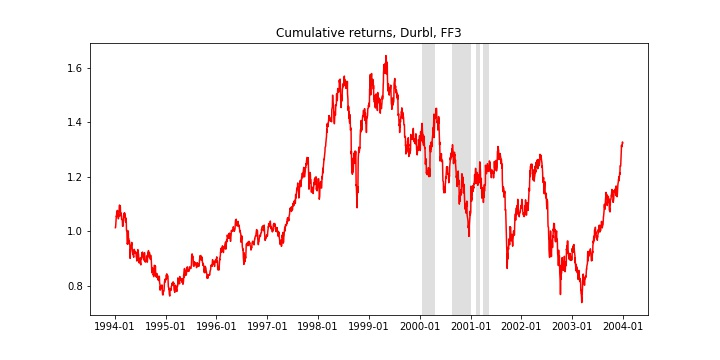
\includegraphics[width=\textwidth]{Durbl/bwunif_full_cumrets_ofint_FF3.jpg}
    \caption*{Rear-facing kernel}
    \label{fig:2}
  \end{subfigure}
  
\end{figure}

\newpage

\begin{figure}

\centering

  \begin{subfigure}[b]{\textwidth}
    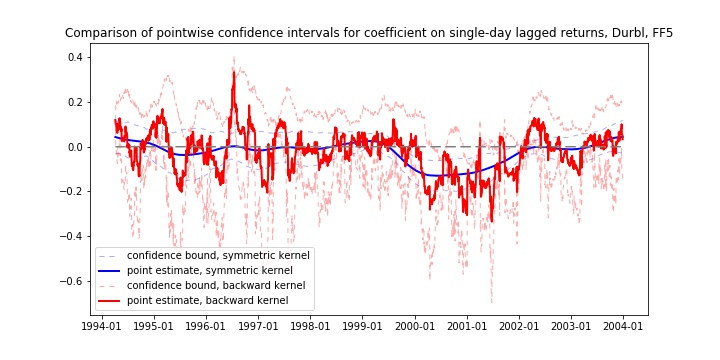
\includegraphics[width=\textwidth]{Durbl/pointwiseCIs_layered_FF5.jpg}
    \label{fig:1}
  \end{subfigure}
  %
  \begin{subfigure}[b]{0.45\textwidth}
    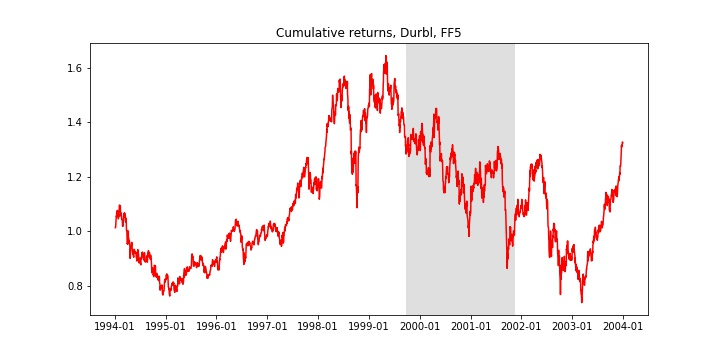
\includegraphics[width=\textwidth]{Durbl/full_cumrets_ofint_FF5.jpg}
    \caption*{Symmetric kernel}
    \label{fig:2}
  \end{subfigure}
  %
   \begin{subfigure}[b]{0.45\textwidth}
    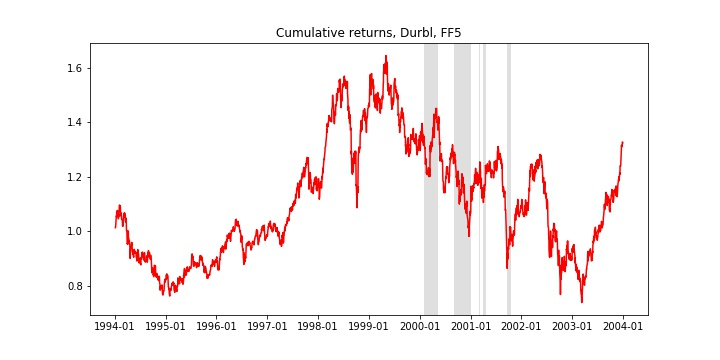
\includegraphics[width=\textwidth]{Durbl/bwunif_full_cumrets_ofint_FF5.jpg}
    \caption*{Rear-facing kernel}
    \label{fig:2}
  \end{subfigure}
  
\end{figure}

\newpage

\begin{figure}

\centering

  \begin{subfigure}[b]{\textwidth}
    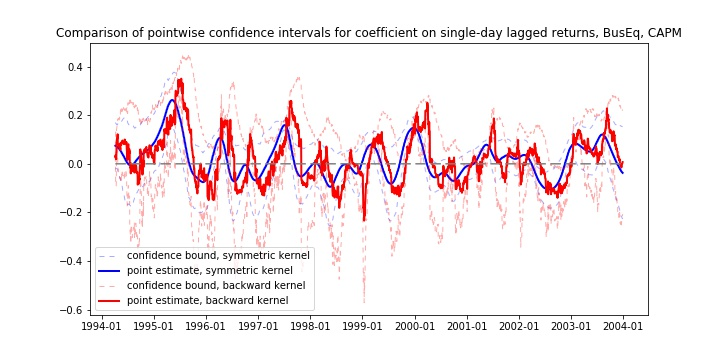
\includegraphics[width=\textwidth]{BusEq/pointwiseCIs_layered_CAPM.jpg}
    \label{fig:1}
  \end{subfigure}
  %
  \begin{subfigure}[b]{0.45\textwidth}
    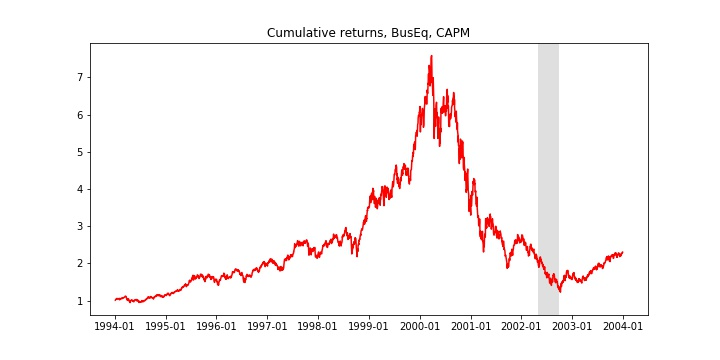
\includegraphics[width=\textwidth]{BusEq/full_cumrets_ofint_CAPM.jpg}
    \caption*{Symmetric kernel}
    \label{fig:2}
  \end{subfigure}
  %
   \begin{subfigure}[b]{0.45\textwidth}
    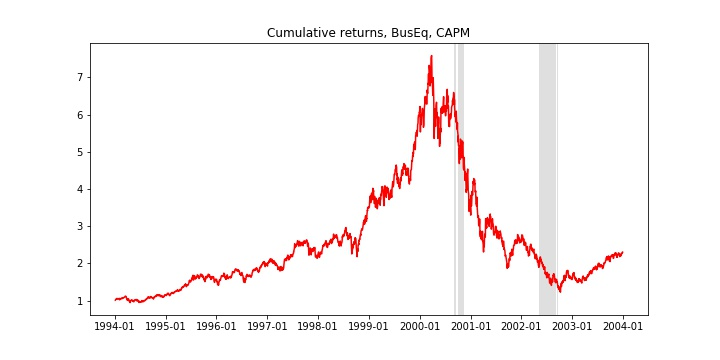
\includegraphics[width=\textwidth]{BusEq/bwunif_full_cumrets_ofint_CAPM.jpg}
    \caption*{Rear-facing kernel}
    \label{fig:2}
  \end{subfigure}
  
\end{figure}

\newpage

\begin{figure}

\centering

  \begin{subfigure}[b]{\textwidth}
    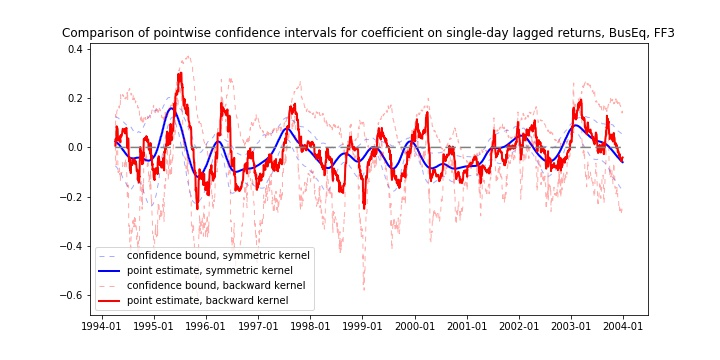
\includegraphics[width=\textwidth]{BusEq/pointwiseCIs_layered_FF3.jpg}
    \label{fig:1}
  \end{subfigure}
  %
  \begin{subfigure}[b]{0.45\textwidth}
    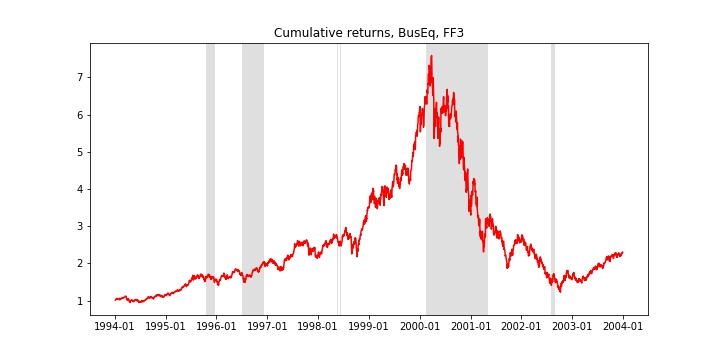
\includegraphics[width=\textwidth]{BusEq/full_cumrets_ofint_FF3.jpg}
    \caption*{Symmetric kernel}
    \label{fig:2}
  \end{subfigure}
  %
   \begin{subfigure}[b]{0.45\textwidth}
    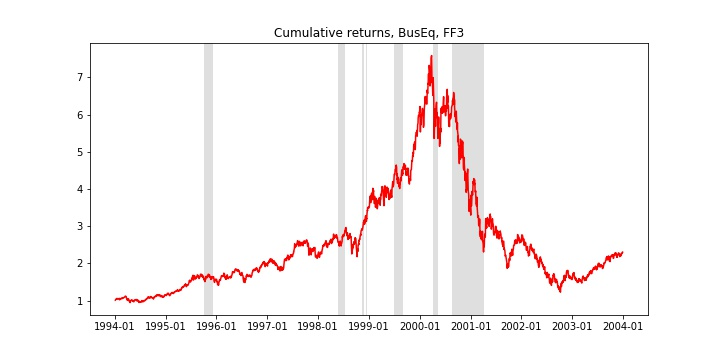
\includegraphics[width=\textwidth]{BusEq/bwunif_full_cumrets_ofint_FF3.jpg}
    \caption*{Rear-facing kernel}
    \label{fig:2}
  \end{subfigure}
  
\end{figure}

\newpage

\begin{figure}

\centering

  \begin{subfigure}[b]{\textwidth}
    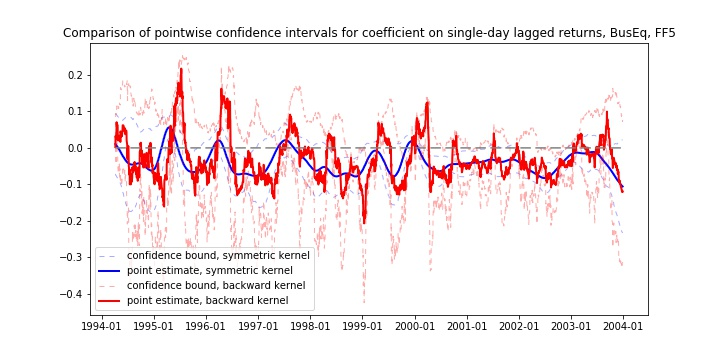
\includegraphics[width=\textwidth]{BusEq/pointwiseCIs_layered_FF5.jpg}
    \label{fig:1}
  \end{subfigure}
  %
  \begin{subfigure}[b]{0.45\textwidth}
    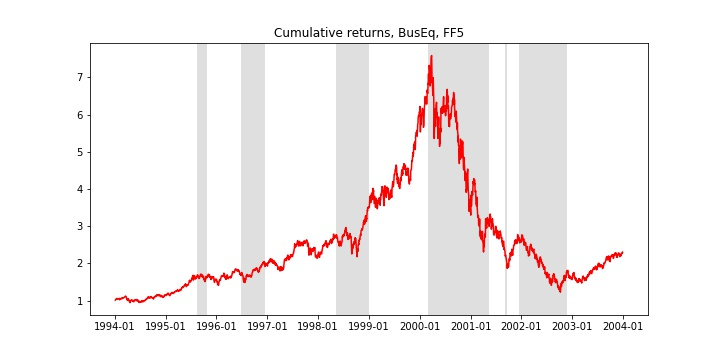
\includegraphics[width=\textwidth]{BusEq/full_cumrets_ofint_FF5.jpg}
    \caption*{Symmetric kernel}
    \label{fig:2}
  \end{subfigure}
  %
   \begin{subfigure}[b]{0.45\textwidth}
    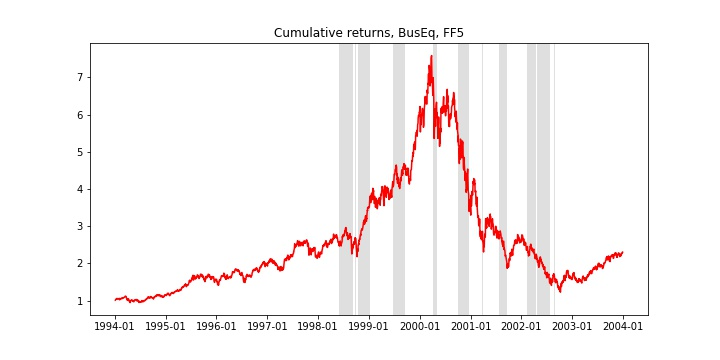
\includegraphics[width=\textwidth]{BusEq/bwunif_full_cumrets_ofint_FF5.jpg}
    \caption*{Rear-facing kernel}
    \label{fig:2}
  \end{subfigure}
  
\end{figure}

\newpage

\begin{figure}

\centering

  \begin{subfigure}[b]{\textwidth}
    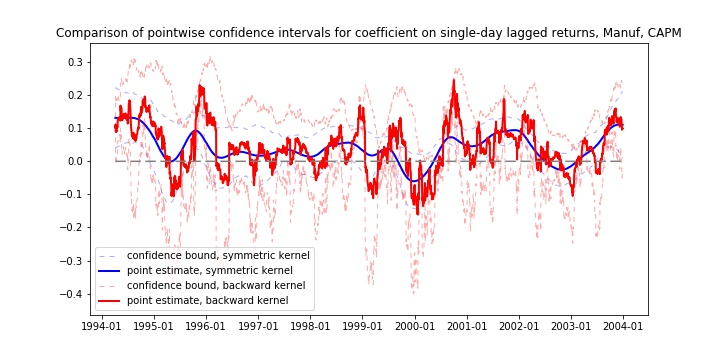
\includegraphics[width=\textwidth]{Manuf/pointwiseCIs_layered_CAPM.jpg}
    \label{fig:1}
  \end{subfigure}
  %
  \begin{subfigure}[b]{0.45\textwidth}
    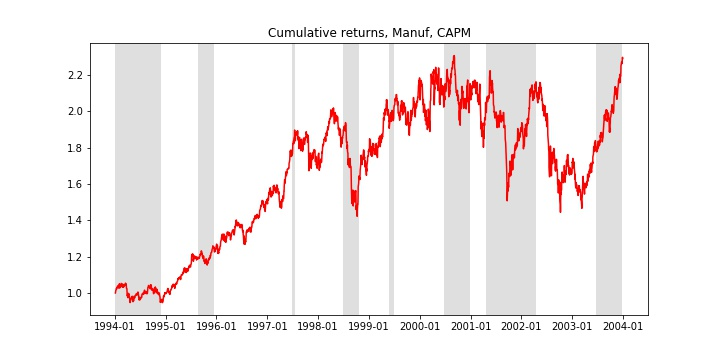
\includegraphics[width=\textwidth]{Manuf/full_cumrets_ofint_CAPM.jpg}
    \caption*{Symmetric kernel}
    \label{fig:2}
  \end{subfigure}
  %
   \begin{subfigure}[b]{0.45\textwidth}
    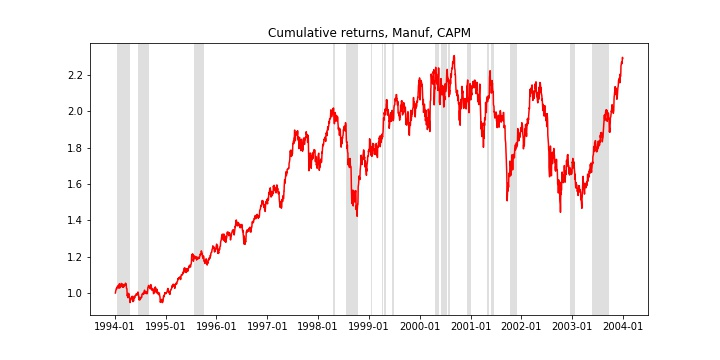
\includegraphics[width=\textwidth]{Manuf/bwunif_full_cumrets_ofint_CAPM.jpg}
    \caption*{Rear-facing kernel}
    \label{fig:2}
  \end{subfigure}
  
\end{figure}

\newpage

\begin{figure}

\centering

  \begin{subfigure}[b]{\textwidth}
    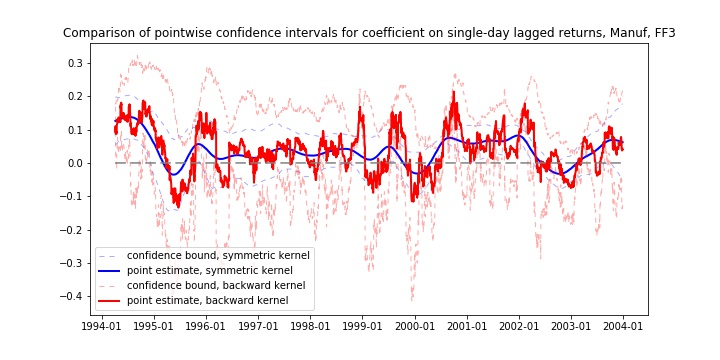
\includegraphics[width=\textwidth]{Manuf/pointwiseCIs_layered_FF3.jpg}
    \label{fig:1}
  \end{subfigure}
  %
  \begin{subfigure}[b]{0.45\textwidth}
    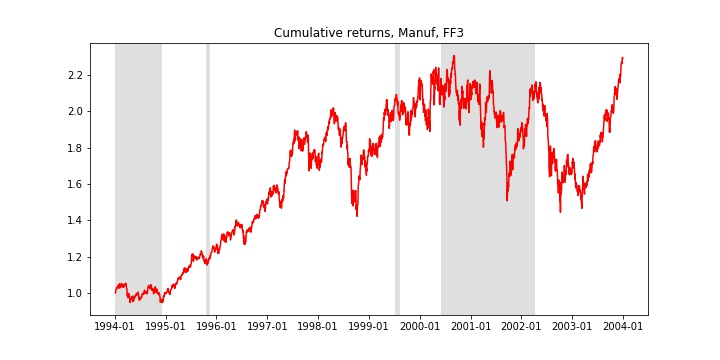
\includegraphics[width=\textwidth]{Manuf/full_cumrets_ofint_FF3.jpg}
    \caption*{Symmetric kernel}
    \label{fig:2}
  \end{subfigure}
  %
   \begin{subfigure}[b]{0.45\textwidth}
    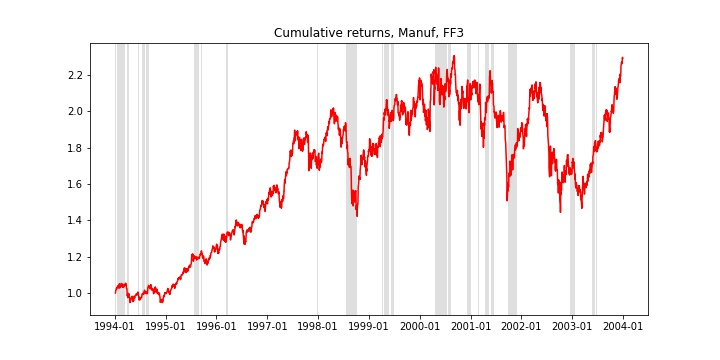
\includegraphics[width=\textwidth]{Manuf/bwunif_full_cumrets_ofint_FF3.jpg}
    \caption*{Rear-facing kernel}
    \label{fig:2}
  \end{subfigure}
  
\end{figure}

\newpage

\begin{figure}

\centering

  \begin{subfigure}[b]{\textwidth}
    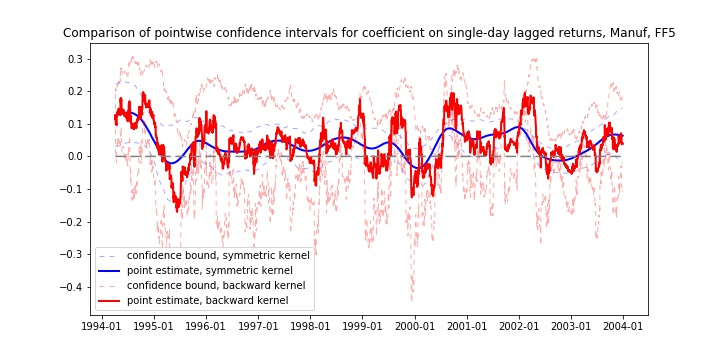
\includegraphics[width=\textwidth]{Manuf/pointwiseCIs_layered_FF5.jpg}
    \label{fig:1}
  \end{subfigure}
  %
  \begin{subfigure}[b]{0.45\textwidth}
    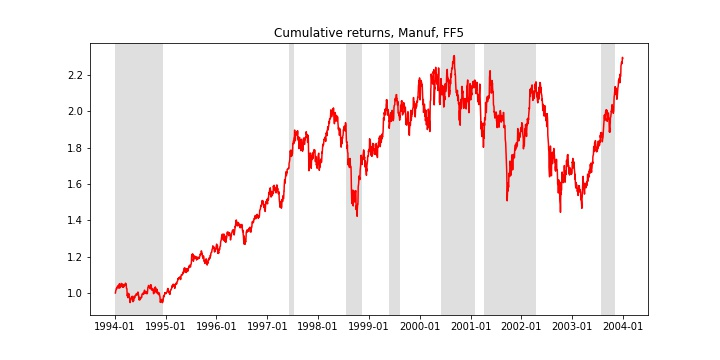
\includegraphics[width=\textwidth]{Manuf/full_cumrets_ofint_FF5.jpg}
    \caption*{Symmetric kernel}
    \label{fig:2}
  \end{subfigure}
  %
   \begin{subfigure}[b]{0.45\textwidth}
    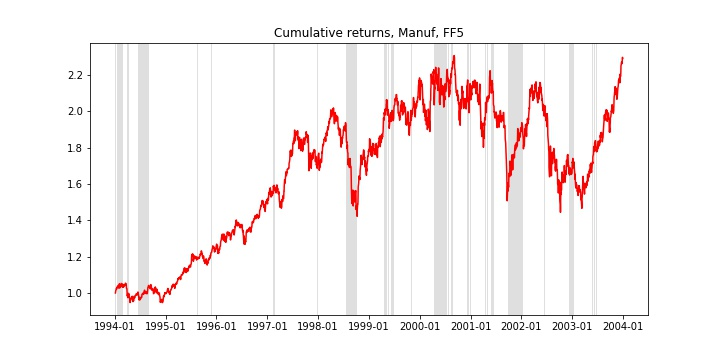
\includegraphics[width=\textwidth]{Manuf/bwunif_full_cumrets_ofint_FF5.jpg}
    \caption*{Rear-facing kernel}
    \label{fig:2}
  \end{subfigure}
  
\end{figure}

\newpage

\begin{figure}

\centering

  \begin{subfigure}[b]{\textwidth}
    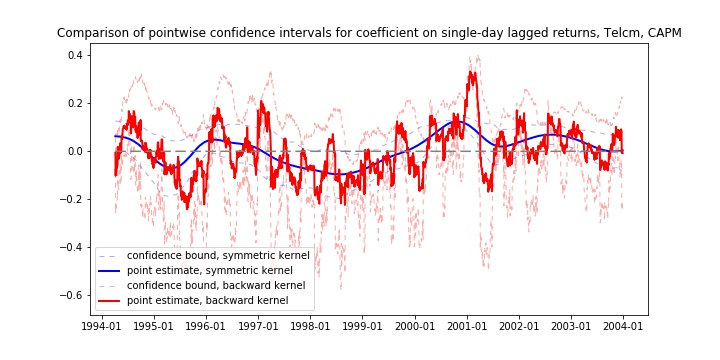
\includegraphics[width=\textwidth]{Telcm/pointwiseCIs_layered_CAPM.jpg}
    \label{fig:1}
  \end{subfigure}
  %
  \begin{subfigure}[b]{0.45\textwidth}
    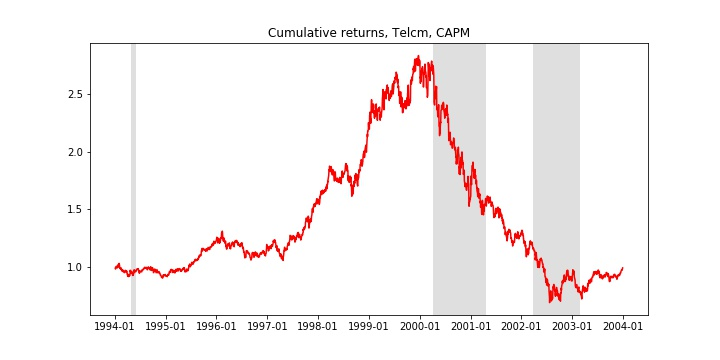
\includegraphics[width=\textwidth]{Telcm/full_cumrets_ofint_CAPM.jpg}
    \caption*{Symmetric kernel}
    \label{fig:2}
  \end{subfigure}
  %
   \begin{subfigure}[b]{0.45\textwidth}
    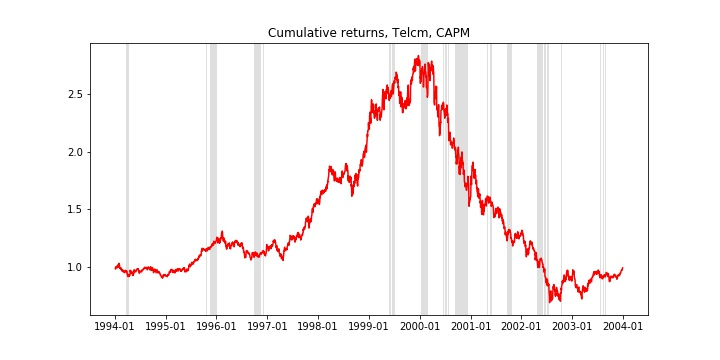
\includegraphics[width=\textwidth]{Telcm/bwunif_full_cumrets_ofint_CAPM.jpg}
    \caption*{Rear-facing kernel}
    \label{fig:2}
  \end{subfigure}
  
\end{figure}

\newpage

\begin{figure}

\centering

  \begin{subfigure}[b]{\textwidth}
    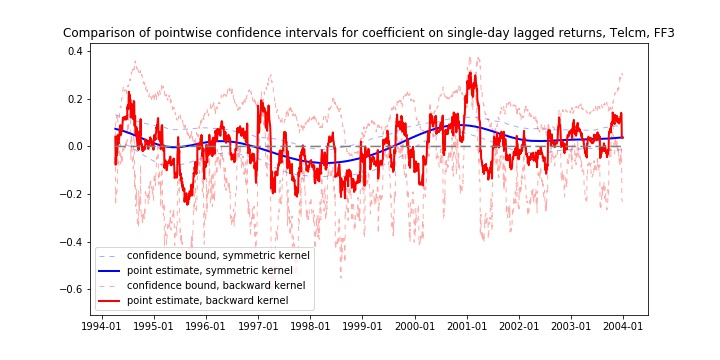
\includegraphics[width=\textwidth]{Telcm/pointwiseCIs_layered_FF3.jpg}
    \label{fig:1}
  \end{subfigure}
  %
  \begin{subfigure}[b]{0.45\textwidth}
    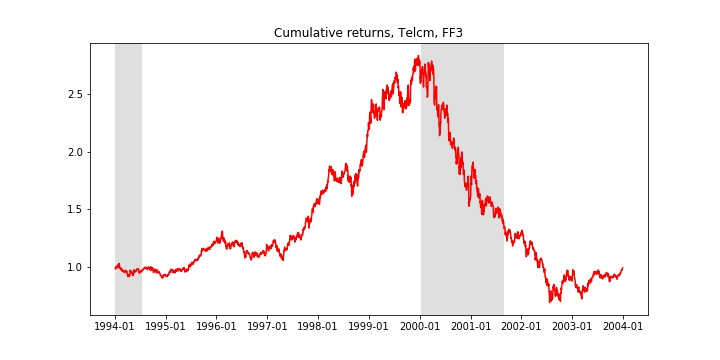
\includegraphics[width=\textwidth]{Telcm/full_cumrets_ofint_FF3.jpg}
    \caption*{Symmetric kernel}
    \label{fig:2}
  \end{subfigure}
  %
   \begin{subfigure}[b]{0.45\textwidth}
    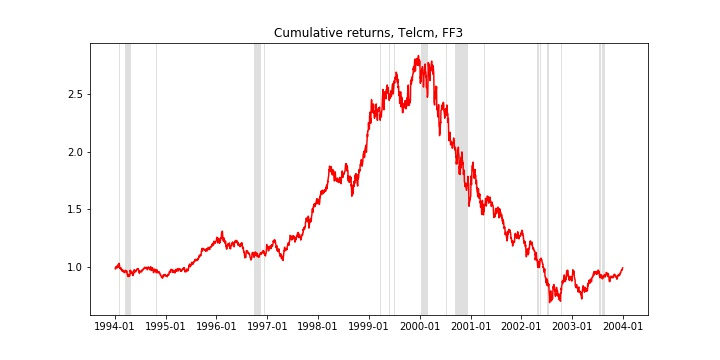
\includegraphics[width=\textwidth]{Telcm/bwunif_full_cumrets_ofint_FF3.jpg}
    \caption*{Rear-facing kernel}
    \label{fig:2}
  \end{subfigure}
  
\end{figure}

\newpage

\begin{figure}

\centering

  \begin{subfigure}[b]{\textwidth}
    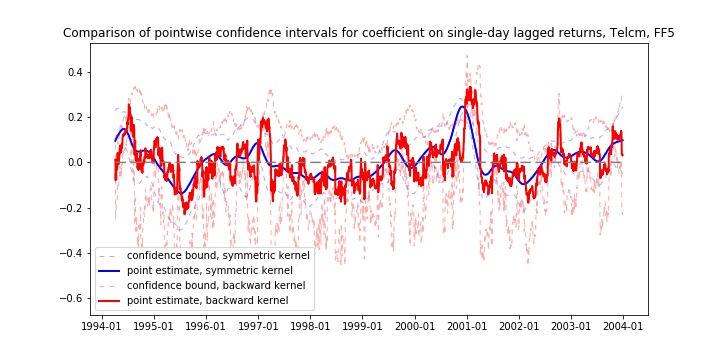
\includegraphics[width=\textwidth]{Telcm/pointwiseCIs_layered_FF5.jpg}
    \label{fig:1}
  \end{subfigure}
  %
  \begin{subfigure}[b]{0.45\textwidth}
    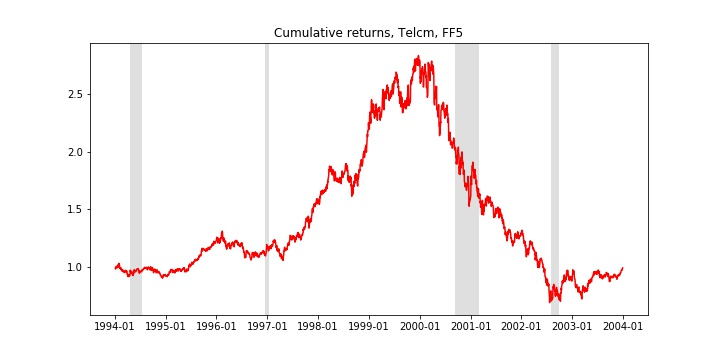
\includegraphics[width=\textwidth]{Telcm/full_cumrets_ofint_FF5.jpg}
    \caption*{Symmetric kernel}
    \label{fig:2}
  \end{subfigure}
  %
   \begin{subfigure}[b]{0.45\textwidth}
    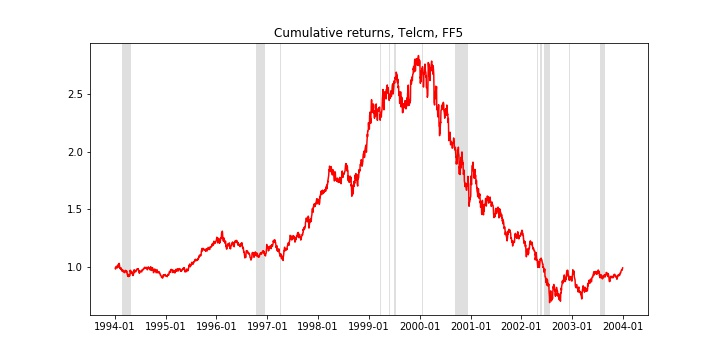
\includegraphics[width=\textwidth]{Telcm/bwunif_full_cumrets_ofint_FF5.jpg}
    \caption*{Rear-facing kernel}
    \label{fig:2}
  \end{subfigure}
  
\end{figure}

\newpage

\begin{figure}

\centering

  \begin{subfigure}[b]{\textwidth}
    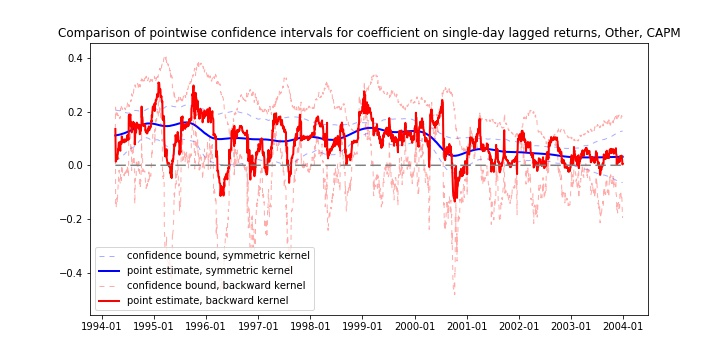
\includegraphics[width=\textwidth]{Other/pointwiseCIs_layered_CAPM.jpg}
    \label{fig:1}
  \end{subfigure}
  %
  \begin{subfigure}[b]{0.45\textwidth}
    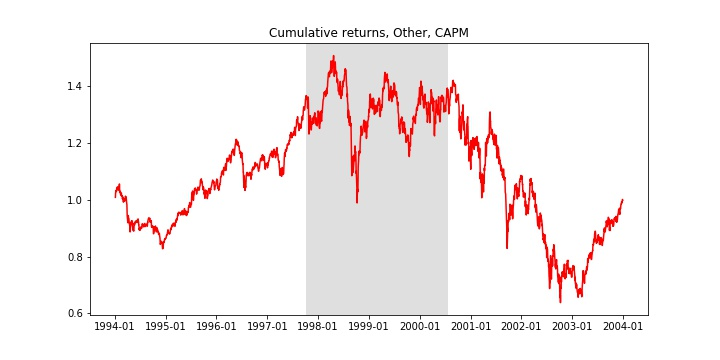
\includegraphics[width=\textwidth]{Other/full_cumrets_ofint_CAPM.jpg}
    \caption*{Symmetric kernel}
    \label{fig:2}
  \end{subfigure}
  %
   \begin{subfigure}[b]{0.45\textwidth}
    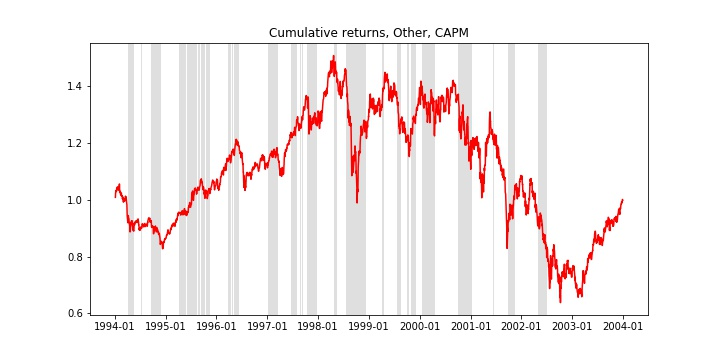
\includegraphics[width=\textwidth]{Other/bwunif_full_cumrets_ofint_CAPM.jpg}
    \caption*{Rear-facing kernel}
    \label{fig:2}
  \end{subfigure}
  
\end{figure}

\newpage

\begin{figure}

\centering

  \begin{subfigure}[b]{\textwidth}
    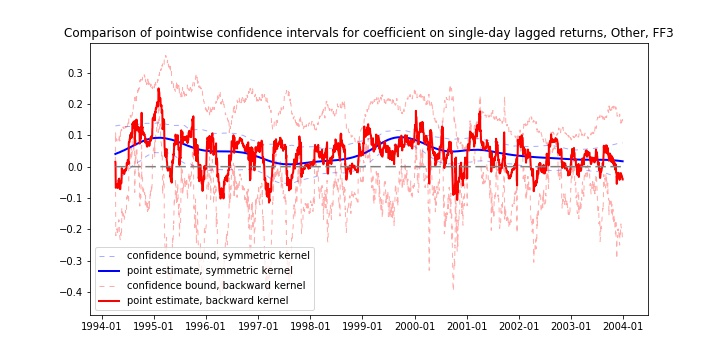
\includegraphics[width=\textwidth]{Other/pointwiseCIs_layered_FF3.jpg}
    \label{fig:1}
  \end{subfigure}
  %
  \begin{subfigure}[b]{0.45\textwidth}
    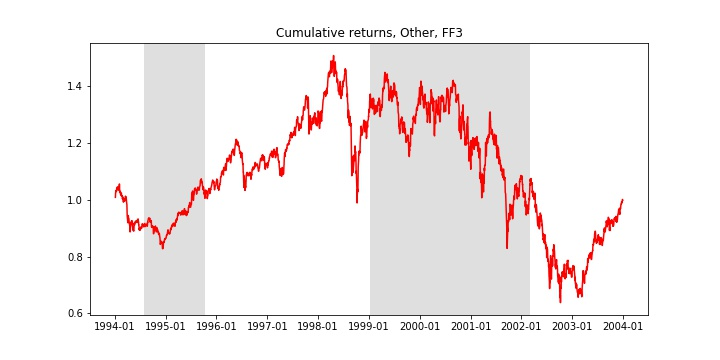
\includegraphics[width=\textwidth]{Other/full_cumrets_ofint_FF3.jpg}
    \caption*{Symmetric kernel}
    \label{fig:2}
  \end{subfigure}
  %
   \begin{subfigure}[b]{0.45\textwidth}
    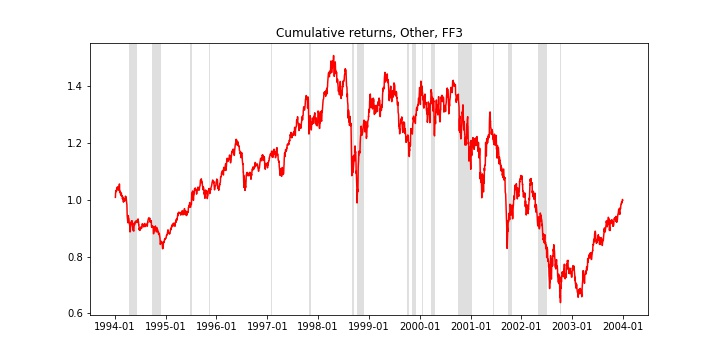
\includegraphics[width=\textwidth]{Other/bwunif_full_cumrets_ofint_FF3.jpg}
    \caption*{Rear-facing kernel}
    \label{fig:2}
  \end{subfigure}
  
\end{figure}

\newpage

\begin{figure}

\centering

  \begin{subfigure}[b]{\textwidth}
    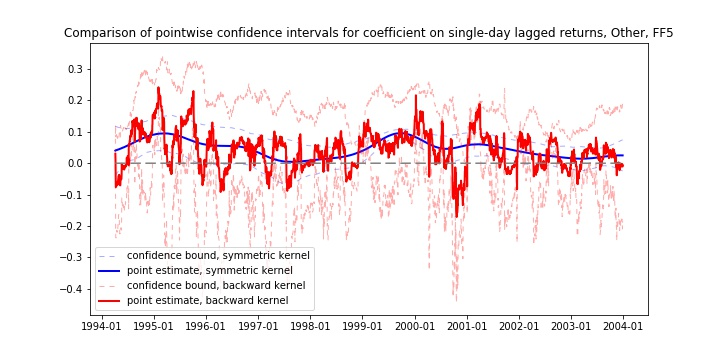
\includegraphics[width=\textwidth]{Other/pointwiseCIs_layered_FF5.jpg}
    \label{fig:1}
  \end{subfigure}
  %
  \begin{subfigure}[b]{0.45\textwidth}
    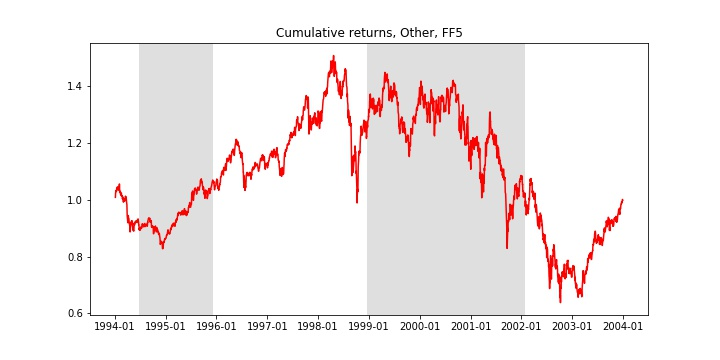
\includegraphics[width=\textwidth]{Other/full_cumrets_ofint_FF5.jpg}
    \caption*{Symmetric kernel}
    \label{fig:2}
  \end{subfigure}
  %
   \begin{subfigure}[b]{0.45\textwidth}
    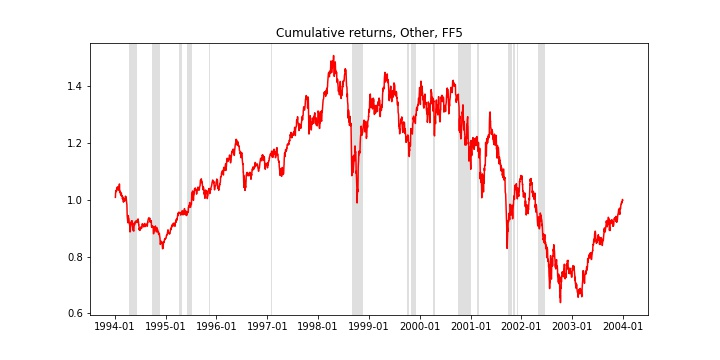
\includegraphics[width=\textwidth]{Other/bwunif_full_cumrets_ofint_FF5.jpg}
    \caption*{Rear-facing kernel}
    \label{fig:2}
  \end{subfigure}
  
\end{figure}

\end{document}